\newcommand\helampl{\mathcal{A}_{\vb*{\lambda}}}

In \cref{chap:stdtech,chap:numunitarity} we were operating on the objects under the assumption that they are Lorentz scalars.
However in QFT scattering amplitudes of particles with spin are not Lorentz scalars,
and the set of all Lorentz structures generated from Feynman diagrams is immensely redundant.
In this chapter we will discuss how amplitudes of any scattering process, 
polarized or not, can be decomposed into a minimal basis of Lorentz-invariant objects.

It is well known that the full physical information about any scattering process is contained in a complete set of \textit{helicity amplitudes} ---
the amplitudes with all external particles' states chosen to have a definite helicity (see the definition in \cref{chap:4dspinhel}).
Being non-redundant and complete representation of physical information, the helicity amplitudes 
enjoy a number of nice properties such as trivialization of gauge-invariance and manifestation of Poincaré symmetry.
On a technical side the consequence is that the helicity amplitudes are expected to have the most compact representation.
And indeed this has been shown to be the case in numerous practical applications (see e.g.\ %
\cite{DeLaurentis:2019phz,Badger:2019djh,Badger:2011yu,Badger:2013gxa,DeFreitas:2004kmi,Gehrmann:2011aa,Gehrmann:2009vu,Glover:2004si,Glover:2003cm,Garland:2002ak,Dunbar:2016aux,Dunbar:2016gjb,Dunbar:2016cxp,Badger:2015lda,Gehrmann:2015bfy,Bern:2003ck,Bern:2002tk,Badger:2018enw,Dunbar2017,Kunszt:1994nq}).

The computation of tree-level helicity amplitudes is a very straight-forward task,
which amounts to simply inserting the corresponding states with definite helicities for each external particle.
The spinor-helicity techniques can be employed to further enhance the computations.
Moving forward to amplitudes with loops,
we are forced to make the dimensionality of space-time formally infinite \cite{Collins:1984xc} 
to regularize divergences.\footnote{other regularization methods are out of the scope of this thesis}
This fact makes both definition and evaluation of helicity amplitudes rather delicate.
It is the purpose of this chapter to present a concise and efficient method of
evaluating multi-loop helicity amplitudes in dimensional regularization,
amenable for numerical applications.

In \cref{sec:helampl_projectors} we briefly review a somewhat standard 
method of obtaining helicity amplitudes through $D$-dimensional projectors,
which can be found in the literature \cite{Garland:2002ak, Moch:2002hm, Glover:2003cm, Glover:2004si,Gehrmann:2009vu,Gehrmann:2011aa}. 
In \cref{sec:helampl_embeding}, 
taking advantage of some insights from \cref{chap:numunitarity},
we show how the tree-level approach of ``simply inserting appropriate external states'' can
be extended to loop amplitudes in the 't Hooft-Veltman (HV) flavor of dimensional regularization.
This allows to dispose of construction of complicated projectors, which
become vary hard to handle for large $(> 4)$ number of particles with spin \cite{Peraro:2019cjj}. 
Another convenient feature of our approach is that it can be applied in a numerical context, such
as evaluation of cuts through off-shell recursion as discussed in \cref{sec:evaluation_of_cuts}.
In \cref{sec:ds_reduction} we discuss how
the efficiency of extraction of the full $D_s$-dependence can be substantially improved
by dimensionally reducing kinematically-independent degrees of freedom in higher dimensions.

\todo{reference spinning particles paper (was for 5 gluon) and another from the guy from MPP} 


\section{Helicity Amplitudes}
\label{sec:HV_helicity_amplitudes}

A helicity amplitude $\helampl$
is defined as an $\mathcal{S}$-matrix element
with external polarization states $\varepsilon_{i}$ chosen to be
helicity eigenstates (for the definition of helicity see \cref{chap:4dspinhel}) with helicities $\vb*{\lambda}=\{\lambda_1,\ldots{},\lambda_N\}$.
Cross-sections obtained from $\Abs{\helampl{}}$ describe
the scattering of polarized particles.
Unpolarized cross-sections can be obtained by summing over the helicities of all external particles
with the help of the completeness relations
\begin{subequations}
  \label{eq:4d_completeness_relations}
  \begin{align}
    \sum_{\lambda=\{+1,-1\}} \varepsilon^\mu_\lambda(p){\varepsilon^\nu_\lambda}^{\star{}}(p)  &= -g^{\mu\nu} + \frac{p^\mu \eta^\nu + p^\nu \eta^\mu}{\sp(p,\eta)}, \\
    \sum_{\lambda=\{+\frac{1}{2},-\frac{1}{2}\}} u^\alpha_\lambda(p){\overline{u}_\lambda^\beta}(p)  &= \qty(\slashed{p}  \pm m\,\mathbb{1})^{\alpha\beta},
  \end{align}
\end{subequations}
for gauge bosons and fermions correspondingly.
The number of $N$-particle helicity amplitudes is thus $2^N$, and
it can be further reduced by taking into an account charge and parity transformations.

The transformation of helicity amplitudes under the Lorentz boosts is completely specified by their 
external states, and is given by the \emph{little group scaling},
\begin{equation}
  \ket{p_i} \to t_i \ket{p_i}, \quad  \sket{p_i} \to \frac{1}{t_i} \ket{p_i} \implies \helampl \to  \qty(\prod_i t_i^{-2\lambda_i}) \helampl,
\end{equation}
where $t_i$ are complex phases.
As expected the squared matrix element $\Abs{\helampl{}}$ is Lorentz-invariant.
With the help of spinor-helicity formalism we can also make any helicity amplitude itself into a scalar
by removing it's \emph{spinor weight} --- a factor which has the same little group scaling
as the helicity amplitude.
Hence the scalar objects we were operating on in \cref{chap:stdtech,chap:dshel} can be the rescaled helicity amplitudes.

We can perturbatively expand helicity amplitudes in the coupling constants as
\begin{equation}
  \helampl =  \helampl^{(0)} + g^2 \helampl^{(1)} + g^4 \helampl^{(2)} + \ldots{},
\end{equation}
with all leading-order couplings absorbed into $\helampl^{(0)}$.
It is then convenient to use the tree helicity amplitude\footnote{if it is not vanishing} $\helampl ^{(0)}$ to remove the spinor weight
of loop amplitudes.
It should be noted that the definition of helicity amplitudes may not depend on a regularization scheme
used to regularize divergences of loop amplitudes. This implies, that 
among the flavors of dimensional regularization only in the ones which consider external particles 
to be in four dimensions the helicity amplitudes can be consistently defined.

%This can be achieved for example by normalizing all amplitudes $A^{L}_N$ with $L\geq1$ by
%a corresponding tree amplitude $A^{0}_N$ 

\section{Form-Factor Decomposition and Projectors}
\label{sec:helampl_projectors}

In this section we review the conceptually simplest way to define helicity amplitudes in dimensional regularization, which is through $D$-dimensional projectors.
This approach has been used in a number of computations \cite{Garland:2002ak, Moch:2002hm, Glover:2003cm, Glover:2004si,Gehrmann:2009vu,Gehrmann:2011aa}.
It's relation to HV scheme and helicity amplitudes has been recently clarified in \cite{Peraro:2019cjj} (see also \cite{Chen:2019wyb}).

One starts with decomposing an amplitude with \emph{unspecified} external states into all possible $D$-dimensional tensor structures $\mathcal{T}_i$ compatible
with symmetries and gauge invariance,
\begin{equation}
  \mathcal{A}  = \sum_{i} \mathcal{T}_i\;A_i.
\end{equation}
For example $\mathcal{T}_i$ can contain object like $\sp(\varepsilon(p_i),p_j)$, $\bar{v}(p_i) \slashed{p}_j u(p_k) $, $\bar{u}(p_i) \slashed{\varepsilon}(p_j) u(p_k)$, etc.
Here $A_i$ are the Lorentz-invariant form-factors.
Then one finds projectors $\mathcal{P}_i$ on $A_i$ from linear combinations of $\mathcal{T}_i$ by solving the equations
\begin{equation} \label{eq:cdr_projectors}
  \mathcal{P}_i [\mathcal{A}] = \qty(\sum_j c_{i,j}(\vb*{x},D) \sum_\text{(states)} \mathcal{T}^{\dagger}_j) \qty[\sum_{k} \mathcal{T}_k A_k] = A_i, 
\end{equation}
for the coefficients $c_{i,j}(\vb*{x},D)$, which are rational functions of external kinematics $\vb*{x}$ and $D$.
Here the state sums are taken to be in $D$ dimensions, which corresponds to working in the CDR scheme.

To extract the helicity amplitudes one then \textit{evaluates} the tensor structures $\mathcal{T}_i$ 
by inserting the corresponding \textit{helicity states in four dimensions} for each of the external particles. 
This is equivalent to switching to the HV scheme.
The procedure uncovers the fact that only particular linear combinations of $A_i$ are relevant,
and the number of these combinations is exactly the number of independent helicity amplitudes, which is
significantly lower than the number of initial tensor structures $\mathcal{T}_i$.

The difficulties of this approach are two-fold:
\begin{enumerate}
  \item The number of initial tensor structures grows very fast with the number of external particles with spin.
    This makes solving the equations \cref{eq:cdr_projectors} for projectors and then applying them to each Feynman diagram very challenging for $N>4$.
  \item The projectors have to be applied to analytic expressions since the external states in $D$ dimensions do not admit any finite numerical representations \cite{Collins:1984xc}.
\end{enumerate}

Since the helicity amplitudes contain the complete physical information, 
the construction of form-factors in  \cref{eq:cdr_projectors} seems to be an unnecessary complication.
And indeed a way to avoid these steps and construct the projector onto helicity amplitudes directly has been suggested recently \cite{Peraro:2019cjj}.
This somewhat mitigates the first issue, but the projectors have to be still applied to analytic expressions.

\section{Helicity Amplitudes in the HV Scheme from Embedding of States}
\label{sec:helampl_embeding}

In this section we explain how multi-loop helicity amplitudes
with vector and spinor external particles can be obtained in dimensional regularization
from appropriate embedding of helicity states into spaces of higher dimensionality $\mathsf{S}_{[D_s]}$.
As in \cref{sec:evaluation_of_cuts}, in this \namecref{chap:dshel} we will denote the dimensionality of particles'
representations as $D_s$.

\todo{
  We build up independently from the projector approach, in the context of dimensional reconstruction. 
  However the correspondence can be straightforwardly established
}

In HV the space-time symmetry group is extended to $\mathrm{SO}(1,D_s-1)$, and the external particles are kept in four dimensions. 
More precisely this means that, like in CDR, the tensor and Clifford algebras are performed in $D_s$ dimensions,
but the completeness relations for external states have to be as in \cref{eq:4d_completeness_relations}. 
In other words the amplitudes in HV transform like their four-dimensional counterpart under $\mathrm{SO}(1,3)$, 
and are invariant under the rotations in $\mathrm{SO}(D_s-4)$. 
This implies that, upon normalizing by an appropriate spinor weight, the helicity amplitudes are scalars of the extended symmetry group $\mathrm{SO}(1,D_s-1)$.
In \cref{chap:numunitarity} we argued that we can use this symmetry to embed the formally infinite-dimensional computation
into a finite one with appropriately chosen integer values of $D^{(L)}$ and $D_s$.
This fact motivates our strategy:
\begin{enumerate}
  \item Consider amplitudes in arbitrary (integer) $D_s > D^{(L)}$ dimensions with fixed external states,
    which have the right little-group behavior with respect to $\mathrm{SO}(1,3) \subset \mathrm{SO}(1,D_s-1)$.
  \item Impose the rotational symmetry in $\mathrm{SO}(D_s-4)$ by combining the degrees of freedom from $\mathsf{S}_{[D_s-4]}$ in
    a suitable way.
  \item Set $D_s\to D$ in the amplitudes obtained from the previous step (which are polynomials in $D_s$).
\end{enumerate}
As we will see shortly, the second step is trivial for vector particles. For fermionic
particles it requires a tensor decomposition similar to the one we discussed in \cref{sec:helampl_projectors},
but enormously simplified by the fact that the indices in  $\mathsf{S}_{[D_s-4]}$ are completely decoupled from kinematics\footnote{
  this applies after the loop integrations are performed, 
  but we can always pull the corresponding projectors into the integrand given that $D_s$ was not set to $D$ yet.
}
and that we can ignore all vector particles.



\subsection{Embedding of Vector States}
\label{sec:embedding_vectors}

Consider the amplitudes for the scattering of massless vector particles.
There are $(D_s - 2)$ states for each particle in $D_s$ dimensions. 
The corresponding polarization sum for a particle with momentum $p$ is 
\begin{equation}
  \sum_{j=1}^{D_s-2} \varepsilon^\mu_j(p){\varepsilon^\nu_j}^{\star{}}(p) = -g_{[4]}^{\mu\nu} + \frac{p^\mu \eta^\nu + p^\nu \eta^\mu}{\sp(p,\eta)} \;-\; g_{[D_s-4]}^{\mu\nu}, 
\end{equation}
where we used $p \in \mathsf{S}_{[4]}$
to make the $(D_s-4)$-dimensional part explicit.
Comparing this to \cref{eq:4d_completeness_relations} we see that we can embed the helicity states as
\begin{align}
  \varepsilon_{1,2}^\mu =
    \begin{dcases}
      \varepsilon^\mu_{+,-}, & \mu\in \mathsf{S}_{[4]},\\
      0, & \mu\in \mathsf{S}_{[D_s-4]},\\
    \end{dcases}
    &&
  \varepsilon_{j}^\mu = \delta^{(j+2)}_\mu, \qfor j\geq 3,
\end{align}
Thus the amplitudes in $D_s$ dimensions with $\varepsilon_{1,2}^\mu$ as external states satisfy the correct little-group scaling trivially.
If we now also take into an account the orthogonality relations 
\begin{align}
  g_{[D_s]}^{\mu\nu} = g^{\mu\nu}_{[4]}+g^{\mu\nu}_{[D_s-4]}, && (g_{[4]})^{\mu\rho}(g_{[D_s-4]})_{\rho\nu} = 0,
      %& (g_{[x]})^{\mu}_\mu =x, \qfor x \in  \{4,D_s,D_s-4\},
\end{align}
we see that these amplitudes are invariants under the rotations in $\mathsf{S}_{[D_s-4]}$.
Hence they are the helicity amplitudes in the HV scheme.
This is, of course, a well-known fact which has been exploited in one-loop computations with numerical generalized
unitary methods \cite{Ellis:2007br,Giele:2008ve}, as well as as 
in the so-called six-dimensional helicity formalism \cite{Bern2011,Cheung:2009dc,Badger:2013gxa,Badger:2017jhb}.

Note that, in contrast to the form-factor decomposition in \cref{sec:helampl_projectors}, we did not need any projectors.

\subsection{Embedding of Spinor States}
\label{sec:embedding_spinors}

We now consider amplitudes with external fermions.
There are $2^{\frac{D_s}{2}-1}$ spinor states in $D_s$ dimensions, 
which can be constructed through the representations of Clifford algebras (see \cref{sec:clifford_algebra_ds}).
The polarization sum with the momentum $p \in \mathsf{S}_{[4]}$ is
\begin{equation}
  \sum_{j=1}^{2^{\frac{D_s}{2}-1}} u^\alpha_j(p){\overline{u}_j^\beta}(p) = \qty(\slashed{p}_{[D_s]}  \pm m\,\mathbb{1}_{[D_s]})^{\alpha\beta} \equiv 
  \qty(\slashed{p}_{[4]} \pm m \cdot \mathbb{1}_{[4]})^{\bar{\alpha}\bar{\beta}} \qty(\mathbb{1}_{[D_s-4]})^{\hat{a}\hat{b}},
\end{equation}
where the indices $\alpha = \bar{\alpha}\otimes\hat{\alpha}$,  $\beta = \bar{\beta}\otimes \hat{\beta}$ are factorized into 
$\{\bar{\alpha},\bar{\beta}\}\in \mathsf{S}_{[4]}$ and $\{\hat{\alpha},\hat{\beta}\}\in \mathsf{S}_{[D_s-4]}$.
Comparing to \cref{eq:4d_completeness_relations}, we see that we can embed the four-dimensional spinors as
\begin{align} \label{eq:fermionicStates}
    \qty(u_{\lambda,i})^{\bar{\alpha}\hat{\alpha}} =  u_{\lambda}^{\bar{\alpha}} \cdot \delta_i^{\hat{\alpha}}, && i = 1,\ldots{},2^{\frac{D_s}{2}-2},
\end{align}
where we replaced the index $j \to \{\lambda, i \}$ to make the four-dimensional helicity $\lambda \in  \{+\frac{1}{2},-\frac{1}{2}\}$ manifest.
Thus the amplitudes in $D_s$ dimensions with any of the spinors $\qty(u_{\lambda,i})^{\bar{\alpha}\hat{\alpha}}$ taken as external fermionic states\footnote{
  The fact the these spinors also satisfy the Dirac equation in $D_s$ dimension can be easily verified.
}
(and with the vector states taken as in \cref{sec:embedding_vectors}) have the correct little-group scaling.
However, as opposed to the case of vector particles, we observe that 
all of the states in \cref{eq:fermionicStates} introduce a \emph{preferred direction} in  $\mathsf{S}_{[D_s-4]}$
via the indices $\hat{\alpha}$.
Hence the corresponding amplitudes are \textbf{not} symmetric under the rotations $\mathrm{SO}(D_s-4)$.
From a different point of view, we have many states with the same helicity, which creates an ambiguity as to what 
should be the helicity amplitude.
On that account, we turn to the tensor decomposition of indices $\hat{\alpha}$.

\subsection{Tensor Decomposition in $D_s-4$}
\label{sec:HelAmplHV}

We decompose an amplitude with external fermions in $D_s$ dimensions as
\begin{equation} \label{eq:tensorDecomposition}
  \mathcal{A} = \sum_n v_n A_n,
\end{equation}
where all spinor indices $\hat{\alpha}_i \in \mathsf{S}_{[D_s-4]}$ (and only them) are absorbed into $v_n$,
and, consequently, $A_n$ are scalars of $\mathsf{S}_{[D_s-4]}$.
In the following we will show how to construct a convenient basis of the tensor structures $v_n$ 
for any number of external fermions.

First we observe that only the spinor chains of the form
\begin{equation} \label{eq:generic_dsm_4_schain}
  u^{\hat{\alpha}}_i \; \qty( \prod_k \gamma^{\mu_k}_{[D_s -4 ]} )^{\hat{\alpha}\hat{\beta}} \; u^{\hat{\beta}}_j \quad\equiv\quad 
  \qty( \prod_k \gamma^{\mu_k}_{[D_s -4 ]} )^{i j},
\end{equation}
with indices $\mu_i \in \mathsf{S}_{[D_s -4]}$ contracted to other spinor chains, contribute to $v_n$.
This is the consequence of the following facts:
\begin{itemize}
  \item Thanks to our choice of states for vector particles, all Lorentz vectors that can be contracted with $\gamma^{\mu_i}_{[D_s]}$
    project them into $\mathsf{S}_{[4]}$:
    \begin{align} \label{eq:trivialTens1}
      a_{\mu}
      \left( \gamma_{[D_s]}^\mu \right)_{\bar{\alpha}\hat{\alpha}}^{\bar{\beta}\hat{\beta}} =
      a_{\mu}\left(\gamma_{[4]}^\mu \right)_{\bar{\alpha}}^{\bar{\beta}} \delta_{\hat{\alpha}}^{\hat{\beta}}\,,
      &&
      a \in \{p_i,\varepsilon_{1,2}(p_i)\}
    \end{align}
    This has an effect that kinematics cannnot enter $v_n$.
  \item Any Lorentz indices inside the same spinor chain can be contracted yielding  
    \begin{equation} \label{eq:trivialTens2}
      \left(\gamma_{[D_s]}^\mu\right)_{\bar{\alpha}\hat{\alpha}}^{\bar{\kappa}\hat{\kappa}}
      \left(\gamma_{[D_s]\mu}^{\phantom{\mu}}\right)_{\bar{\kappa}\hat{\kappa}}^{\bar{\beta}\hat{\beta}}
      =D_s~\delta_{\bar{\alpha}}^{\bar{\beta}}\delta_{\hat{\alpha}}^{\hat{\beta}}\,.
    \end{equation} 
  \item Due to the factorized representation of the Clifford algebra (see \cref{eqn:cliffordrecursion}), any spinor chain can be written in a factorized form.
\end{itemize}
Non-trivial tensors $v_n$ are thus obtained by contracting
Lorentz indices between multiple chains of  matrice $\gamma_{[D_s-4]}$.
Some examples of possible $v_n$ are
\begin{equation}
  \begin{aligned}
    & \delta^{i_1}_{j_1} \delta^{i_2}_{j_2},\\
    & (\gamma_{[D_s-4]}^{\mu_1} )_{i_1}^{j_1} (\gamma_{[D_s-4]\mu_1}^{\phantom{\mu}})_{i_2}^{j_2}, \\
    & (\gamma_{\mu_1[D_s-4]}^{\phantom{\mu}} )_{i_1}^{j_1} (\gamma_{[D_s-4]}^{\mu_1}\gamma_{[D_s-4]}^{\mu_2} )_{i_2}^{j_2} (\gamma_{[D_s-4]\mu_2}^{\phantom{\mu}})_{i_3}^{j_3},\\
    & \qquad \vdots{}
  \end{aligned}
\end{equation}

Evidently to construct a basis of tensor structures $v_n$ we can decompose each of the spinor chains entering it
into the standard basis of anti-symmetrized products of gamma-matrices (see e.g.\ \cite{Veltman:1988au}),
\begin{align}\label{eq:basisGammaChainDs}
\gamma_{[D_s-4]}^{\mu_1 \ldots \mu_n} = \frac{1}{n!} \sum_{ \sigma\in S_n} \sgn(\sigma) \gamma_{[D_s-4]}^{\mu_{\sigma(1)}} \ldots \gamma_{[D_s-4]}^{\mu_{\sigma(n)}}\,,
\end{align}
where $S_n$ denotes the set of all permutations of $n$
integers and $\sgn(\sigma)$ the signature of the permutation
$\sigma\in S_n$.
It can be shown (see \cref{sec:identities}), that the
projectors $\mathcal{P}_n$ onto $v_n$ can be constructed from the conjugated tensors $v_n^\dagger$ as
\begin{align} \label{eq:dsm_4_projectors}
  \mathcal{P}_n [v_m] \coloneqq \prod_{s_1}^{n_s} \Tr_s \qty(v_n^\dagger v_m) = c_n(D_s)~\delta_{n m},  %&& c_n = \frac{(D_s-4)!\,n!}{(D_s-4-n)!},
\end{align}
with the traces are taken over each of $n_s$ spinor chains, and we drop the irrelevant total factor of $\qty(\Tr\mathbb{1}_{[D_s -4 ]})^{n_s}$.
The coefficients $c_n$ can be computed for each $n_s$ combinatorially, as demonstrated in \cref{eq:cnCalc}.
We emphasize that, unlike the projectors in \cref{sec:helampl_projectors}, the ones in \cref{eq:dsm_4_projectors}
operate on the explicitly-represented objects, hence can be evaluated numerically.
We now consider two examples.

\paragraph{One pair of external fermions.}
As a first and trivial example we consider an amplitude with one pair of external fermions (and any number of external gauge bosons). 
There is only a single chain of matrices $\gamma_{[D_s-4]}$, so
there is only a single term in the decomposition of \cref{eq:tensorDecomposition},
\begin{equation}\label{eq:decompqqbar}
  \mathcal{A} =v_0\,A_0\,,\qquad \textrm{with}\quad (v_0)_{\hat{\alpha}}^{\hat{\beta}}=\delta_{\hat{\alpha}}^{\hat{\beta}}\,.
\end{equation}
\paragraph{Two pairs of distinct fermions.}
As a second example we consider an amplitude with two fermion pairs of different flavors, (and any number of gauge bosons). 
The basis $\{v_n\}$ consists of contraction between two spinor chains of the form \cref{eq:generic_dsm_4_schain}:
\begin{align}
  \begin{split} \label{eqn:4qtensors}
    (v_0)_{j_1j_2}^{i_1i_2}   = &
    \delta_{j_1}^{i_1} \delta_{j_2}^{i_2}\,, \\
    (v_1)_{j_1j_2}^{i_1i_2}=
    &(\gamma_{[D_s-4]}^{\mu_1} )_{j_1}^{i_1} 
    (\gamma_{[D_s-4]\mu_1}^{\phantom{\mu}})_{j_2}^{i_2}\,, \\
    & \vdots\\
    (v_k)_{j_1j_2}^{i_1i_2}=
    &(\gamma_{[D_s-4]}^{\mu_1 \ldots  \mu_m})_{j_1}^{i_1}
    (\gamma_{[D_s-4]\mu_1 \ldots \mu_m}^{\phantom{\mu}})_{j_2}^{i_2}\,,\\
    & \vdots\,
  \end{split}
\end{align}
The number of elements in the basis $\{v_n\}$ depends on $D_s$,
and is infinite for non-integer $D_s$ (because the basis of the Clifford algebra \cref{eq:basisGammaChainDs} is infinite).
But for any given number of loops $L$ only a finite number of basis elements $n^{(L)}\coloneqq \dim\{v_n\}$ can appear.
This number can be found from inspecting the diagrams without external gauge bosons 
with maximal number of propagators.
For instance we have $n^{(0)}=0$, $n^{(1)}=3$ and $n^{(2)}=5$.

Each coefficient $A_n$ in the decomposition of \cref{eq:tensorDecomposition} satisfies our desiderata 
of the HV amplitudes from \cref{sec:HV_helicity_amplitudes}, so, in principle, we need to determine all of them to obtain the full amplitude.
In the next section we argue that, at least to NNLO, it is not the case, 
and all physically-relevant information can be extracted from just one coefficient.  

\subsection{Relevant Coefficients}
\label{sec:relevant_tensors}

It was shown in \cite{Weinzierl:2011uz} that for NNLO computations only the $\order{\eps^0}$ terms of the 
\emph{finite remainders} $\mathcal{F}^{(1)}$ and $\mathcal{F}^{(2)}$ of one- and two-loop amplitudes are required.
They are defined by subtracting the universal divergent structure of one- and two-loop amplitudes, 
\begin{subequations}
  \begin{align}
    \label{eq:F0}
    \mathcal{F}^{(0)} &\coloneqq \mathcal{A}^{(0)}, \\ 
     \label{eq:F1}
    \mathcal{F}^{(1)} &\coloneqq \mathcal{A}^{(1)} - \mathbf{I}^{(1)} \mathcal{A}^{(0)}, \\ 
     \label{eq:F2}
    \mathcal{F}^{(2)} &\coloneqq \mathcal{A}^{(2)}  - \mathbf{I}^{(1)} \mathcal{A}^{(1)} - \mathbf{I}^{(2)} \mathcal{A}^{(0)}.
  \end{align}
\end{subequations}
The operators $\mathbf{I}^{(1)}$ and $\mathbf{I}^{(2)}$ can be found in \cite{Catani:1998bh,Sterman:2002qn,Becher:2009cu,Gardi:2009qi}.
Here for convenience we also introduced a finite remainder for tree amplitudes, which is simply an alias for the amplitude itself.
We can expand both sides of \cref{eq:F0,eq:F1,eq:F2} in terms of tensor structures of \cref{eq:tensorDecomposition}
to get the corresponding coefficients $\mathcal{F}^{(i)}_n$ of the finite remainders.
\todo{possibly comment on why we can do this} 
The cross-section is obtained by squaring the finite remainders, possibly multiplied by some
finite operator $\mathbf{F}$ (we refer to \cite{Weinzierl:2011uz} for details),
\begin{equation} \label{eq:Fsq}
  \Ree{\mathcal{F}^{(i)}}{\mathbf{F}\mathcal{F}^{(j)}} = \sum_m\sum_n\; \mathcal{P}_m \qty[v_n]  \; \Ree{\mathcal{F}^{(i)}_m}{\mathbf{F}\mathcal{F}^{(j)}_n} = 
     \sum_n c_n \; \Ree{\mathcal{F}^{(i)}_n}{\mathbf{F}\mathcal{F}^{(j)}_n},
\end{equation}
where in the last equality we used \cref{eq:dsm_4_projectors}.
For non-identical pairs of fermions\footnote{we discuss identical fermions below} 
the first element of the basis $\{v_n\}$ is
\begin{equation}
  v_0  = \delta^{\hat{\alpha}_1}_{\hat{\beta}_1}\cdots \delta^{\hat{\alpha}_{n_s}}_{\hat{\beta}_{n_s}},
\end{equation}
and the corresponding coefficient $c_0 = 1$.
As demonstrated in \cref{sec:identities}, the coefficients of all other tensor structures
contribute to higher orders in $\eps$ when we set $D_s\to 4-2\eps$,
\begin{equation}
  c_i=\order{\eps}, \qfor i\geq 1,
\end{equation}
We can drop all $\order{\eps}$ terms in \cref{eq:Fsq}.
Thus we conclude that all we need to know is the coefficient of $v_0$.


\subsubsection{Identical Fermions}
To illustrate how to handle the cases with identical fermions,
we consider an amplitude with two pairs of fermions with the same flavor. 
It can be constructed by anti-symmetrizing the corresponding amplitude with distinct flavors.
In this way, we start from the basis in \cref{eqn:4qtensors},
and extend it with anti-symmetrized tensors $\{\tilde v_n\}$ as
\begin{equation}\label{eq:basisIdentical}
	(\tilde v_n)_{j_1j_2}^{i_1i_2}= (v_n)_{j_1j_2}^{i_2i_1}\,,
\end{equation}
so our basis is now $\{v_n\}\cup \{\tilde{v}_n\}$.
It satisfies the following properties:
\begin{equation}\label{eq:dualBasisIdentical}
  \mathcal{P}_n[v_m]= c_n \delta_{m n}\,,\qquad
  \mathcal{\tilde{P}}_n[\tilde{v}_m]= \tilde{c}_n \delta_{m n}\,,\qquad
  \mathcal{P}_n[\tilde{v}_m] = \delta_{m 0}\,\delta_{n 0}+\mathcal{O}(\epsilon)\,.
\end{equation}
The coefficients in the first two equations are the same as for the case of distinct fermions. 
We do not provide the closed form for the coefficients in the last equation, but
the fact that they are always proportional to $(D_s-4)$ can be straightforwardly verified.

Now consider the interference between the two-loop finite remainder and 
the corresponding tree amplitude, which are anti-symmetrized over flavors individually,
\begin{multline}
  \qty(\mathcal{F}^{(0)} - \mathsf{f}\circ\mathcal{F}^{(0)})^\dagger \cdot 
    \qty(\mathcal{F}^{(2)} - \mathsf{f}\circ\mathcal{F}^{(2)}) = \\
    \qty(\mathcal{P}_0\qty[\mathcal{F}^{(0)}] - \mathcal{P}_0\qty[\mathsf{f}\circ\mathcal{F}^{(0)}])^\dagger \cdot 
    \qty( \mathcal{P}_0\qty[\mathcal{F}^{(2)}] - \mathcal{P}_0\qty[\mathsf{f}\circ\mathcal{F}^{(2)}]) ~+~ \order{\epsilon}.
\end{multline}
Here the application of $f\circ$ exchanges the flavors. 
On the right hand side we used the identities from \cref{eq:dualBasisIdentical} to
show that, to $\order{\epsilon}$, 
we can anti-symmetrize the coefficients $\mathcal{F}_0$ of the remainders.
And the latter are computed as in the case of distinguishable fermions.

As another interesting application of these observations, we can explain why 
two different results for the two-loop helicity amplitudes of the four-quark scattering in QCD
from \cite{Glover:2004si} and \cite{DeFreitas:2004kmi} give the same
value for the finite remainder\footnote{The fact that the finite remainders agree was recognized by the authors of \cite{DeFreitas:2004kmi}}.
The authors of the former computed 
\[
  \mathcal{P}_0\qty[\mathcal{A}^{(2)}(q,\bar{q},Q,\bar{Q})],
\]
while the authors of the latter computed
\[
  \tilde{\mathcal{P}}_0\qty[\mathcal{A}^{(2)}(q,\bar{q},Q,\bar{Q})].
\]
Clearly these results will not be the same. 
However, taking into an account the \cref{eq:dualBasisIdentical}, we get
\[
  \mathcal{P}_0\qty[\mathcal{F}^{(2)}] = \tilde{\mathcal{P}}_0\qty[\mathcal{F}^{(2)}] ~+~ \order{\epsilon}.
\]

\subsection{Chiral Couplings}

It is well known, that dimensional regularization fails to regularize chiral theories consistently
(see e.g.\ \cite{Larin:1993tq,Boughezal:2019xpp,Jegerlehner:2000dz,Bonneau:1980yb,Bruque:2018bmy,Baikov:1991qz,Kreimer:1989ke}).
More colloquially this problem is known as ``the $\gamma_5$ problem'', because it is it's analytic
continuation to $D$ dimensions which causes contradictions explicitly.
The dimensional regularization can still be employed in these models, 
but some additional manual interference is required in some cases. 

In this thesis we only consider two-loop amplitudes in pure QCD, so we do not have to explore the issue. 
Nevertheless we would like to comment on how our method of extraction of helicity amplitudes might be affected by it.
First of all, we emphasize that we \emph{did not} construct a new flavor of dimensional regularization,
and our results are that of the HV scheme.  So the discussion found in the literature applies to our results without modifications.
To this end, a prescription with  the ``four-dimensional'' $\gamma_5$ \cite{tHooft:1972tcz,Breitenlohner:1977hr,Larin:1993tq},
\[\commutator{\gamma_{5}}{\gamma^{\mu}_{[D_s]}}=0, \quad \forall \mu\geq 4,\]
can be trivially incorporated in our approach with the following:
\[
  \qty(\gamma_{5[D_s]})^{\bar{\alpha}\hat{\alpha}}_{\bar{\beta}\hat{\beta}} = \qty(\gamma^\star_{[4]})^{\bar{\alpha}}_{\bar{\beta}}\,\delta^{\hat{\alpha}}_{\hat{\beta}},
\]
and an explicit addition of counter-term contributions might be required.
Finally, it is worth mentioning that using the ``anti-commuting'' $\gamma_5$, that is
\[
  \anticommutator{\gamma_{5}}{\gamma^{\mu}_{[D_s]}}=0, \quad \forall \mu, \qquad\Longleftrightarrow\qquad \gamma_{5[D_s]} \equiv \gamma^\star_{[D_s]},
\]
in combination with dimensional reconstruction is not possible, since
in this case the amplitudes behave non-smoothly as functions of $D_s$ at all integer values.

\subsection{Discussion}
\label{sec:dshel_discussion}


\todo{Compared to the form-factor decomposition in \cref{sec:helampl_projectors} it is easy to see that $v_0$ is the coefficient in HV scheme} 
It is then rather straight-forward to see that the coefficient $A_0$ of $v_0$ coincides with
the amplitude obtained following the prescription of \cref{sec:helampl_projectors}, as well
as the result of the``'t Hooft-Veltman algebra'' implemented in \cite{Cullen2010}.

In agreement with the prescription of ref.~\cite{Anger:2018ove}.

\todo{Validated extremely well by reproducing all the results computed from the form-factor decomposition} 
In summarry, as long as phenomenological applications concerned, we only need to consider $v_0$.

\todo{Important transition between schemes} 
The two schemes are consistent,
in that their contributions to NNLO computations can be related by known
transition rules~\cite{Broggio:2015dga}, but as we
shall see below the HV scheme introduces some simplification in
the calculation.

The idea of embedding external states into higher-dimensional spaces to obtain
helicity amplitudes in dimensional regularization is not new. 
It has been employed in one-loop numerical generalized
unitary methods \cite{Ellis:2007br,Giele:2008ve}, as well as as 
the so-called six-dimensional helicity formalism \cite{Bern2011,Cheung:2009dc,Badger:2013gxa,Badger:2017jhb} for two loops.
However the embedding of fermionic states, in particular any number of them,
and the relation to the HV scheme were largely glossed over,
which caused some confusion in the past.

For example if one takes a ``single'' embedding of external quarks \todo{expand on this, reference an explicit state} ,
one effectively considers an amplitude polarized in $\mathsf{S}_{[D_s-4]}$ ,
so the computation carried out in this way do not correspond to the HV scheme.
Strictly speaking then the arguments we used for the dimension of embedding of loop momenta are invalidated.
\todo{list of cases when single embedding fails} 

At the integrand level this manifests itself as appearing of explicit components of $\ell^\mu_{i[D-4]}$, not as scalar products $\mu_{ij}$ (see \cref{sec:PartialFractions}).
At one loop this was observed as ``odd $\mu$ powers'' in \cite{Fazio:2014xea,Badger:2017gta}.
It can be shown that if there are less than two \emph{massive} quark pairs, simply discarding 
the odd $\mu$ powers leads to the HV results to $\order{\eps^0}$.
However the differences will appear starting from $\order{\epsilon}$ for any amplitude
with more than two quark pairs, massive or not.
From two-loop onwards the differences will appear already in the poles in $\epsilon$. 
For example the single embedding was used in \cite{DeFreitas:2004kmi} for the computation of two-loop four-quark amplitudes,
and the result for the amplitude differs significantly from our results and the result of \cite{Glover:2004si}.
In \cref{sec:relevant_tensors} we explained why the finite remainders agree.

\todo{All particles can be massive, nothing changes, but the little-group scaling is replaced by the q-helicity scaling.} 


 

\section{$D_s$-Dependence From Dimensional Reduction}
\label{sec:ds_reduction}
Here we explain how to improve the extraction of $D_s$-dependence.
This is crucial for amplitudes with external fermions due to the exponential scaling of the representation.


The amplitudes $A$ defined in eq.~\eqref{eq:defAmpsTens} are polynomials in $D_s$,
\begin{equation}
  A(D_s) = \sum_{i=0}^{N} \mathcal{K}_i~D_s^{i}\ ,
  \label{eq:ds-poly}
\end{equation}
where $N$, the maximal power of $D_s$, 
varies depending on the process, the loop order, and the choice of tensor structure 
in eq.~\eqref{eq:tensorDecomposition}.
For the amplitudes considered in this paper $N\leq2$.
In this section we will suppress all arguments of $A$ and only keep track of the 
dependence on~$D_s$.
%
In a numerical framework, $A(D_s)$ can only be evaluated for integer $D_s$ values for which 
the particle states are well defined.
To be able to set $D_s=4-2\epsilon$ in the HV scheme, the knowledge of the coefficients $\mathcal{K}_i$ is required.
One way to obtain them is to reconstruct the polynomial \eqref{eq:ds-poly} from
a sample of $(N+1)$ integer values of $D_s$.
This procedure is known as dimensional reconstruction \cite{Giele:2008ve} and has  previously been applied
in \cite{Ellis:2008ir,Boughezal:2011br,Abreu:2017xsl,Abreu:2017hqn}.

While being generic and straightforward to implement, this approach has drawbacks which
become particularly evident in amplitudes with fermions.
%
The dimension of the spinor representation scales exponentially (as $2^{D_s/2}$) with $D_s$,
as opposed to the linear scaling of the vector representation.
Furthermore, the external spinor states with definite helicity can be embedded consistently
only for even values of $D_s$,
which pushes the sample values higher compared to the case of vector particles in the loops.
Beyond the obvious detrimental effect on the numerical complexity, the dimensionality of the
spinor representation determines the number of terms entering the evaluation of the traces
to obtain the helicity amplitudes through  eq.~\eqref{eq:defAmpsTens}. For
the case of amplitudes with multiple external quark pairs this makes the computation
of traces unnecessarily time consuming.

These considerations motivate the search for more efficient alternatives to dimensional
reconstruction. Here we employ one such alternative, based on the idea of
dimensional reduction, which has recently been presented in ref.~\cite{Anger:2018ove} 
and already applied to the computation of one-loop amplitudes in ref.~\cite{Anger:2017glm}.
In the remainder of this section we give a brief overview of this method 
and refer the reader to ref.~\cite{Anger:2018ove} for more technical details.

We start by rearranging eq.~\eqref{eq:ds-poly} in the following way:
\begin{equation}
  A(D_s) = \sum_{i=0}^{N} \tilde{\mathcal{K}}_i~(D_s-D_0)^{i},
  \label{eq:ds-poly-alt}
\end{equation}
where $D_0$ is some \textit{base} dimension, and the coefficients $\tilde{\mathcal{K}}_i$
can be obtained by a linear transformation of the coefficients $\mathcal{K}_i$ in eq.~\eqref{eq:ds-poly}.
It turns out that, given a suitable choice of $D_0$,
the dependence of $A(D_s)$ on degrees of freedom higher than $D_0$ can
be captured in a kinematic-independent way.  
This observation allows one to analytically separate this
dependence, and thus evaluate each coefficient $\tilde{\mathcal{K}}_i$
directly. Furthermore, these evaluations are then performed in the base
dimension $D_0$, resulting in spinor representations of much lower dimensionality
compared to those encountered in the framework of dimensional reconstruction.

For reasons that will become clear shortly, one chooses the base
dimension $D_0$ to be the minimal dimension which allows to embed 
all loop-momentum components without introducing new relations.
For two-loop amplitudes we have $D_0=6$, and we
shall specialize to this case henceforth. We write the metric tensor as
a direct sum,
  \begin{align}
    \label{eq:ds-split-metric}
    g^{\mu\nu}_{[D_s]}  = g^{\mu\nu}_{[D_s-6]} + g^{\mu\nu}_{[6]},  \qquad
    g^{\mu\nu}_{[D_s-6]}g^{\phantom{\mu\nu}}_{\mu\nu\,[6]} = 0\,,
  \end{align}
  and the gamma matrices as a direct product 
  (see e.g.\ \cite{Collins:1984xc,Kreuzer:susylectures}),
\begin{equation}
  (\gamma_{[D_s]}^\mu)_{a\kappa}^{\,b\lambda}  = \left\{ 
    \begin{array}{ll} 
      \left(\gamma_{[6]}^\mu\right)_a^{\;b} \,
      \delta_\kappa^\lambda\,, &\quad  0\le\mu \le 5 \,,\\&\\
      \left(\gamma^\star_{[6]}\right)_a^{\;b} 
      \left(\gamma_{[D_s-6]}^{(\mu-6)}\right)_\kappa^{\;\lambda}\,, 
      &\quad \mu \geq 6 \,,
    \end{array}
    \right.
    \label{eq:ds-gamma}
\end{equation}
where $\gamma^\star_{[6]}$ is a six-dimensional analogue of $\gamma_5$ in four dimensions, i.e.\ $\{\gamma^\star_{[6]},\gamma_{[6]}^\mu\} = 0$ for all $\mu \in \{0,5\}$, and $(\gamma^\star_{[6]})^2 = 1$.
The product representation allows us to factorize any chain of gamma matrices into a product of $6$- and $D_s-6$-dimensional gamma-matrix chains.
Then, using the fact that the trace of a direct product of two matrices is the product of their traces,
we can split the traces required to obtain the coefficients of tensor structures in eq.~\eqref{eq:tensorDecomposition}
as follows:
\begin{equation}
  \Tr\left(\prod_{\mu_i\in \mathcal{G}}\gamma^{\mu_i}_{[D_s]}\right) =
  \Tr\left(\prod_{\mu_i\in \tilde{\mathcal{G}}}\gamma^{\mu_i}_{[D_s-6]}\right) \cdot
  \Tr\left(\prod_{\mu_i\in \mathcal{G}}\gamma^{\mathfrak{I}(\mu_i)}_{[6]}\right),
  \label{eq:ds-split-traces}
\end{equation}
where the product on the left-hand side is over a sequence $\mathcal{G}$ of $D_s$-dimensional Lorentz indices,
$\tilde{\mathcal{G}} = \{ \mu_i \in \mathcal{G} ~\vert~ \mu_i \geq 6 \}$, and the map $\mathfrak{I}$ is defined as
\begin{equation}
  \mathfrak{I} : \mu \to
    \begin{cases}
      \mu, & 0\le\mu \le 5\,, \\
      \star, & \mu \geq 6\,.
    \end{cases}
\end{equation}
The traces of $\prod_{\mu_i\in\tilde{\mathcal{G}}}\gamma^{\mu_i}_{[D_s-6]}$ can be 
evaluated analytically using well-known Clifford algebra identities,
which produce sums of products of $g^{\mu_i\mu_j}_{[D_s-6]}$.
%
The crucial observation is that the only object to be contracted with the indices beyond 
$(D_s-6)$ is $g^{\mu\nu}_{[D_s-6]}$.
This is ensured by our choice of the base dimension.
These indices then always contribute terms of the form $g^\mu_{[D_s-6]\mu} = (D_s-6)$, 
generating contributions to the coefficients $\tilde{\mathcal{K}}_i$ with $i>0$ 
in eq.~\eqref{eq:ds-poly-alt}. At this point, all degrees of freedom beyond $(D_s-6)$
are traded for polynomials in $(D_s-6)$ with integer factors, and the coefficients
$\tilde{\mathcal{K}}_i$ are expressed in terms of six-dimensional objects only.

\todo{Put examples of tree and 1-loop.}

\subsection{Dimensionally Reduced Feynman Rules}
\label{sec:DsFeynRules}
In the table~\ref{tab:Ds-FeynRules} we list the color-ordered Feynman rules for vertices involving the scalar particles introduced in section~\ref{sec:Ds}.
The $(D_s-6)$-dimensional part of these rules can be fully contracted in each Feynman diagram yielding kinematic-independent factors.
\begin{table}[h]
  \centering
  \begin{minipage}[t]{0.4\textwidth}
    \small
  \begin{tabular}{cl}
    $\vcenter{\hbox{\hspace{-2ex}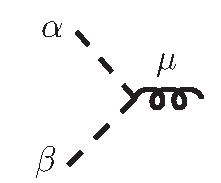
\includegraphics[width=13ex]{figures/Vssg}}}$ & $ \frac{i}{\sqrt{2}}(p_2-p_1)^\mu~ g^{\alpha\beta}_{[D_s-6]}$ \\
    $\vcenter{\hbox{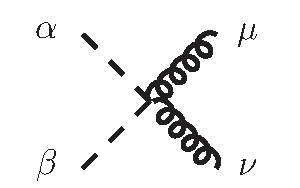
\includegraphics[width=15ex]{figures/Vssgg}}}$ & $ -\frac{i}{2}~g^{\mu\nu}_{[6]}~g^{\alpha\beta}_{[D_s-6]}$ \\
    $\vcenter{\hbox{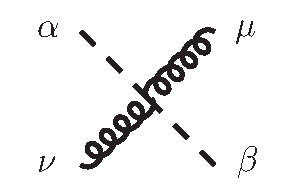
\includegraphics[width=15ex]{figures/Vsgsg}}}$ & $ i~g^{\mu\nu}_{[6]}~g^{\alpha\beta}_{[D_s-6]}$ \\
  \end{tabular}
  \end{minipage}
  \quad
  \begin{minipage}[t]{0.5\textwidth}
    \small
  \begin{tabular}{cl}
    $\vcenter{\hbox{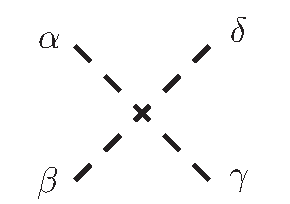
\includegraphics[width=15ex]{figures/Vssss1}}}$ &
      $
      \begin{aligned}
        i~g^{\alpha\gamma}_{[D_s-6]} g^{\beta\delta}_{[D_s-6]} - ~ & \\
                \frac{i}{2}~(g^{\alpha\beta}_{[D_s-6]} g^{\gamma\delta}_{[D_s-6]} & + g^{\alpha\delta}_{[D_s-6]} g^{\beta\gamma}_{[D_s-6]})
      \end{aligned}
      $ \\
        $\vcenter{\hbox{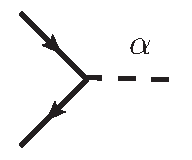
\includegraphics[width=11ex]{figures/VqqsR}}}$ & $- \frac{i}{\sqrt{2}}~\gamma^\star_{[6]} \gamma^\alpha_{[D_s-6]}$ \\
        $\vcenter{\hbox{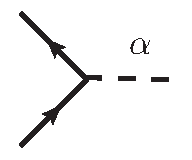
\includegraphics[width=11ex]{figures/VqqsL}}}$ & $ \frac{i}{\sqrt{2}}~\gamma^\star_{[6]} \gamma^\alpha_{[D_s-6]}$ \\
  \end{tabular}
  \end{minipage}
  \caption{Color-ordered Feynman rules for vertices with scalar particles explicitly introduced by dimensional reduction of gluons.}
  \label{tab:Ds-FeynRules}
\end{table}

\FloatBarrier

From a Feynman diagrammatic perspective, the contributions to the
coefficients of the polynomial in $(D_s-6)$
can be represented by introducing a scalar particle. 
The Feynman rules associated to this particle can be readily
derived from dimensional reduction of the original Feynman rules of the
theory \cite{Bern:2002zk,Badger:2013gxa,Giele:2008ve,Anger:2018ove} by
applying the relations \eqref{eq:ds-split-metric} and \eqref{eq:ds-gamma}.
We list them in the appendix \ref{sec:DsFeynRules} for convenience.
To illustrate this procedure we now give an example. 
Consider a decomposition of a Feynman diagram with $D_s$-dimensional particles on the 
left-hand side of figure~\ref{fig:ds-example-diagram}. The four non-vanishing 
contributions after evaluating partial traces and contracting all 
$(D_s-6)$-dimensional indices are shown on the right-hand side, 
where the scalars are introduced to represent what remains of these contractions.

\begin{figure}
  \newlength\diagramWidth
  \setlength{\diagramWidth}{18ex}
  \centering
  \begin{align*}
    \vcenter{\hbox{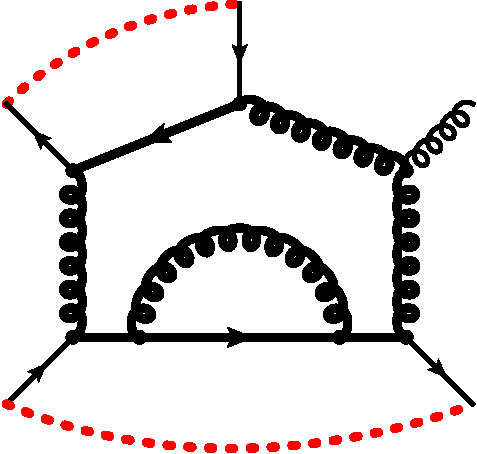
\includegraphics[width=\diagramWidth]{figures/Ds-example_B.pdf}}} \hspace{-10ex} & \hspace{15ex} = \hspace{6ex}
    \vcenter{\hbox{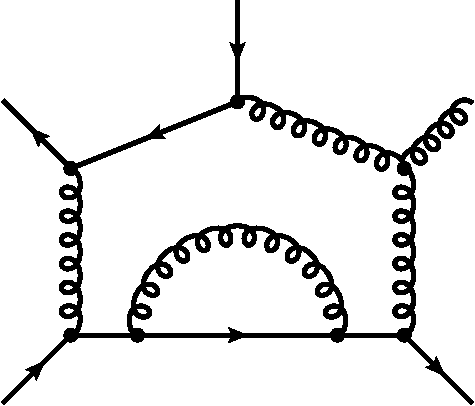
\includegraphics[width=\diagramWidth]{figures/Ds-example.pdf}}} \quad +\\
    \Big(~ &
    \vcenter{\hbox{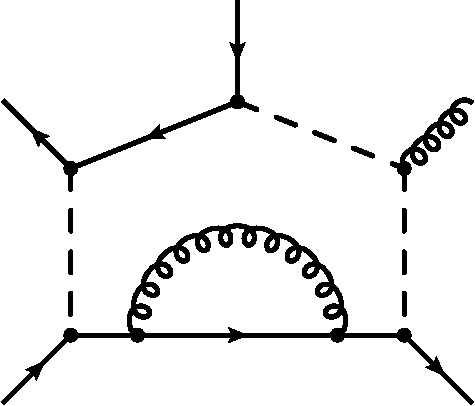
\includegraphics[width=\diagramWidth]{figures/Ds-example-1-1.pdf}}} \quad+\quad
    \vcenter{\hbox{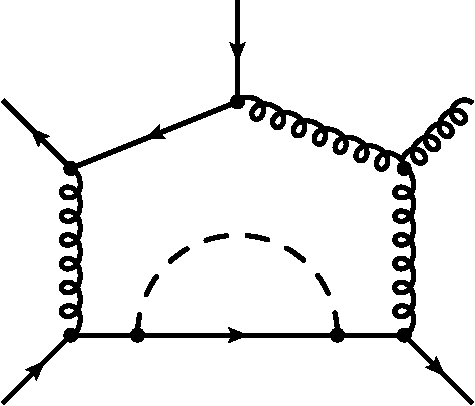
\includegraphics[width=\diagramWidth]{figures/Ds-example-1-2.pdf}}}
    ~\Big) ~\cdot~ (D_s-6) \quad +\\
    &
    \vcenter{\hbox{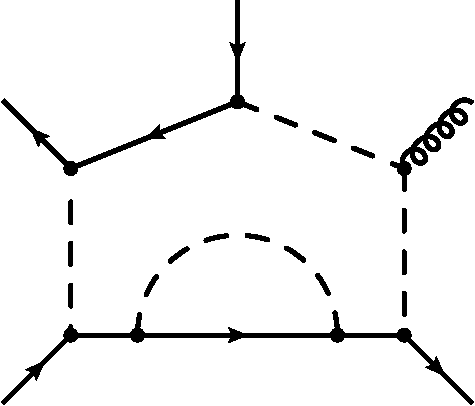
\includegraphics[width=\diagramWidth]{figures/Ds-example-2.pdf}}}
    ~\cdot~ (D_s-6)^2,
  \end{align*}
  \caption{Example of diagrams with scalar particles,
    representing the contributions to the coefficients of $\tilde{\mathcal{K}}_i$ in eq.~\eqref{eq:ds-poly-alt}.
    The thick lines in the diagram on the left-hand side represent particles in arbitrary $D_s$ dimensions.
    The (red) dashed lines connecting external-quark lines represent the traces required to obtain the coefficient of the tensor structure of eq.~\eqref{eq:defAmpsTensb}.
    All particles on the right-hand side are in six dimensions.}
  \label{fig:ds-example-diagram}
\end{figure}


We would like to conclude this section with some remarks.
First, the remaining non-trivial traces of eq.~\eqref{eq:ds-split-traces},
i.e.\ those of $\prod_k\gamma^{\mu_k}_{[6]}$, cannot be simplified generically
as the indices appear contracted with the loop momenta at the integrand level.
We evaluate them by the direct summation over a specially constructed set of external states
(in an analogous way to the sums performed in~\cite{Abreu:2018jgq} 
for dimensional reconstruction).
Secondly, in the absence of fermions in the loops, this method coincides with the so called
six-dimensional formalism employed in refs.~\cite{Badger:2013gxa,Badger:2017jhb}, and can 
thus be viewed as an extension thereof to amplitudes with fermions.
Finally, we note that the method presented in this section can be straightforwardly
generalized to higher number of loops by adjusting the base dimension $D_0$,
as well as to the extraction of coefficients of different tensor structures in 
eq.~\eqref{eq:tensorDecomposition}.



\subsection{Unitarity-Compatible Implementation}
decomposition of trees through simplified off-shell recursion.
    Collecting $(D_s-6)$ powers and factors. Implementation in process libraries.

    \todo{Use tree example here}



